%% IMPORTANT: Once working, run latex 3 times to get listoffigures to work

%% Be sure to check spelling!

%% Put **your** name and the proper due date in place

%% Copy the lstlisting and figure code as many times as you need
%% Be sure to put in your own file names if appropriate

%% Note that the \epsfig commands are currently commented out - until the
%%%% files exist, processing this code without them will result in an error
%%%% so leave the comments until you have created the graphics files!

\documentclass{article}
\usepackage{array}      % allows m{width} in tabulars for vertical centering
\usepackage{amsmath}    % load AMS-Math package
\usepackage{epsfig}     % allows PostScript files
\usepackage{listings}   % allows lstlisting environment
\usepackage{moreverb}   % allows listinginput environment
\usepackage{vmargin}    % allows better margins
\setpapersize{USletter} % sets the paper size
\setmarginsrb{1in}{0.5in}{1in}{0.2in}{12pt}{11mm}{0pt}{11mm} %sets margins 
\begin{document}
\begin{center}
\rule{6.5in}{0.5mm}\\~\\
{\bf \large EGR 103L - Fall 2016}\\~\\
{\huge \bf Laboratory 3 - Program Control and Functions}\\~\\
CEMAL YAGCIOGLU (cy111)\\
Lab 05,Wednesda 11.45 AM - 2.35 PM \\
25 September, 2016\\~\\
{\small I understand and have adhered to all the tenets of the Duke
  Community Standard in completing every part of this assignment.  I
  understand that a violation of any part of the Standard on any part
  of this assignment can result in failure of this assignment, failure
  of this course, and/or suspension from Duke University.} 
\rule{6.5in}{0.5mm}\\
\end{center}
\tableofcontents
\listoffigures
\pagebreak

\section{Chapra Problem 2.6}
The equation for the charge on the capacitor\cite[p.~44]{Chapra} is:
\begin{align*}
q(t)=q_0 e^{-Rt/(2L)}\mathrm{cos}\Bigg[\sqrt{\frac{1}{LC}-\Big(\frac{R}{2L}\Big)^2}t\Bigg]
\end{align*}
The graph of 'Charge on the Capacitor Over Time' has a sinusoidal curve with a decreasing range over time. As the time passes the oscillation of charge on the capacitor decreases, and gets closer to a constant.

\section{Based on Chapra Problem 2.22}
The equations for the butterfly curve\cite[p.~47]{Chapra} are:
\begin{align*}
x &= \mathrm{sin}(t)\bigg(e^{\mathrm{cos}t}-2\mathrm{cos}4t-\mathrm{sin}^5\frac{t}{12}\bigg)\\
y &= \mathrm{cos}(t)\bigg(e^{\mathrm{cos}t}-2\mathrm{cos}4t-\mathrm{sin}^5\frac{t}{12}\bigg)
\end{align*}
As they have both x and y  have sinusoidal graphes, together they form a equation for 'r', radius from the origin point that changes its direction and magnitude according to the functions. Graph is reflective over y-axis, and r has a larger value while x is positive. Due to these two factors, the curve for y positive values is larger compared to the curve for y negative values, creating a figure to a butterfly.  

\section{Chapra Problem 3.10}
% Commentary on where and what the greatest displacements are should
% be here.
Minimum displacement is at the point (8.7076,-32.741).Thus, it is -32.741 feet. Maximum displacement is at the point (5.7019,195.32).Thus, it is 195.32 feet. 
% The final plot is in the Appendix. 
% The full text of the function and script are in the Appendix

\section{Palm Problem 4.44}
\renewcommand{\arraystretch}{1.3}
The $a$ and $b$ values for six gases are, from
references \cite{Palm} and \cite{LibreTexts} and alphabetically by gas name:
\begin{center}
\begin{tabular}{ccc}\hline
Gas & a($\mathrm{L}^2$-atm/$\mathrm{mo}l^2$) & b(L/mol)\\\hline
Chlorine,C$\mathrm{l}_2$ & 6.49 & 0.0562\\
Ammonia,N$\mathrm{H}_3$ & 4.225 & 0.03713\\
Carbon dioxide,C$\mathrm{O}_2$ & 3.59 & 0.0427\\
Oxygen,$\mathrm{O}_2$ & 1.36 & 0.0427\\
Helium,He & 0.0341 & 0.0237\\
Hydrogen,$\mathrm{H}_2$ & 0.244 & 0.0266\\\hline
\end{tabular}
\end{center}
A graph of pressures for the above gases at $T=$300K and specific volumes $\hat{V}$ between 1 and 2 L/mol is presented in Figure \ref{PressureGraph} on page
\pageref{PressureGraph}.  The pressure for each gas comes from
the following function given in Palm \cite[p.~215]{Palm}:
\begin{align*}
P=\frac{RT}{\hat{V}-b}-\frac{a}{\hat{V}^2}
\end{align*}

\section{Palm Problem 4.19}
See Table \ref{LeapYearsTest} on page \pageref{LeapYearsTest}.
% Nothing else to say, really!

\pagebreak
\appendix
\section{Codes}
% Put the name of your file in the subsection name 
% and the listinginput input
% Be sure to include the community standard in codes!

% Add \pagebreaks if they make sense

% Put the files in the same order as the problems; generally, 
% scripts will come first followed by any functions called
% by those scripts.

\subsection{PlotCharge.m}
\listinginput[1]{1}{PlotCharge.m}

\subsection{Charge.m}
\listinginput[1]{1}{Charge.m}

\subsection{RunButterfly.m}
\listinginput[1]{1}{RunButterfly.m}

\subsection{Butterfly.m}
\listinginput[1]{1}{Butterfly.m}

\subsection{TestSingularity.m}
\listinginput[1]{1}{TestSingularity.m}

\subsection{BeamDisplacement.m}
\listinginput[1]{1}{BeamDisplacement.m}

\subsection{GraphPressures.m}
\listinginput[1]{1}{GraphPressures.m}

\subsection{VanDerWaals.m}
\listinginput[1]{1}{VanDerWaals.m}

\subsection{LeapYears.m}
\listinginput[1]{1}{LeapYears.m}
\clearpage % start Diary on new page

\section{Diary}
\begin{table}[htb!]
\listinginput[1]{1}{ChargeDiary.txt}
\begin{center}
\caption{Output from TestCharge.m\label{ChargeTest}}
\end{center}
\end{table}

\begin{table}[htb!]
\listinginput[1]{1}{LeapDiary.txt}
\begin{center}
\caption{Output from TestLeapYear.m\label{LeapYearsTest}}
\end{center}
\end{table}
\clearpage % start Figures on new page

\section{Figures}
% Don't forget to take out % on epsfig lines!

\begin{figure}[ht!]
\begin{center}
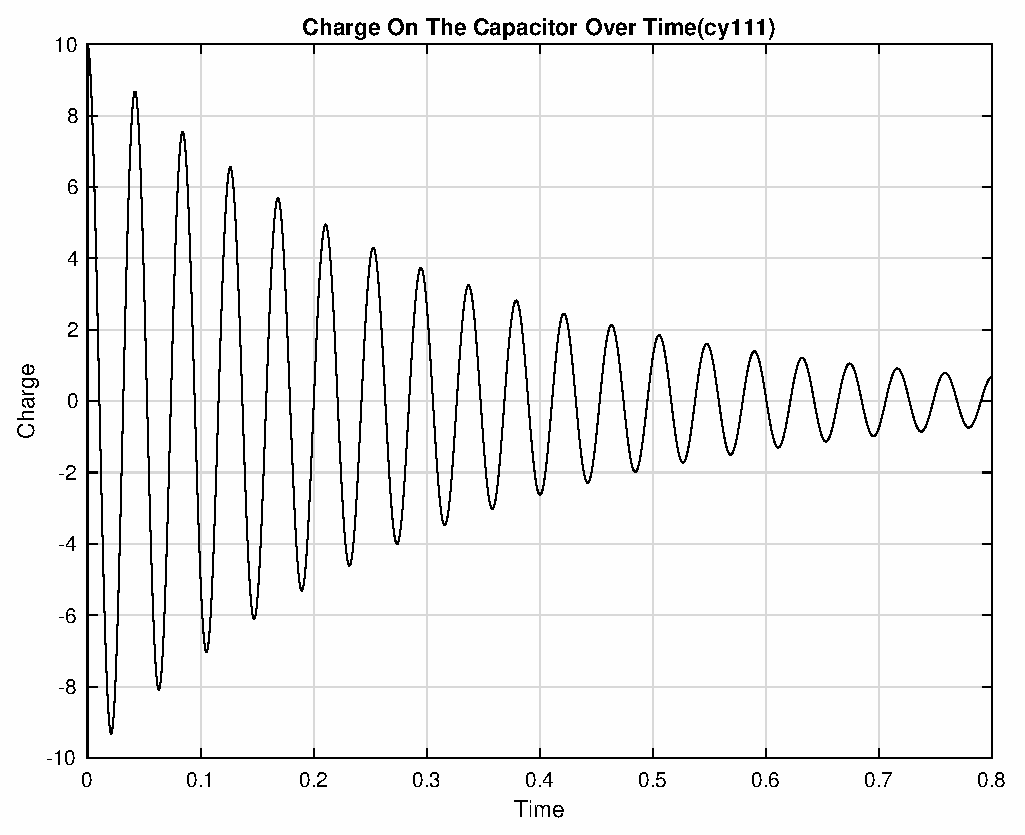
\epsfig{file=ChargePlot.eps, width=4.5in}
\caption{Plot for Chapra 2.9.\label{ChargeGraph}}
\end{center}
\end{figure}

\begin{figure}[ht!]
\begin{center}
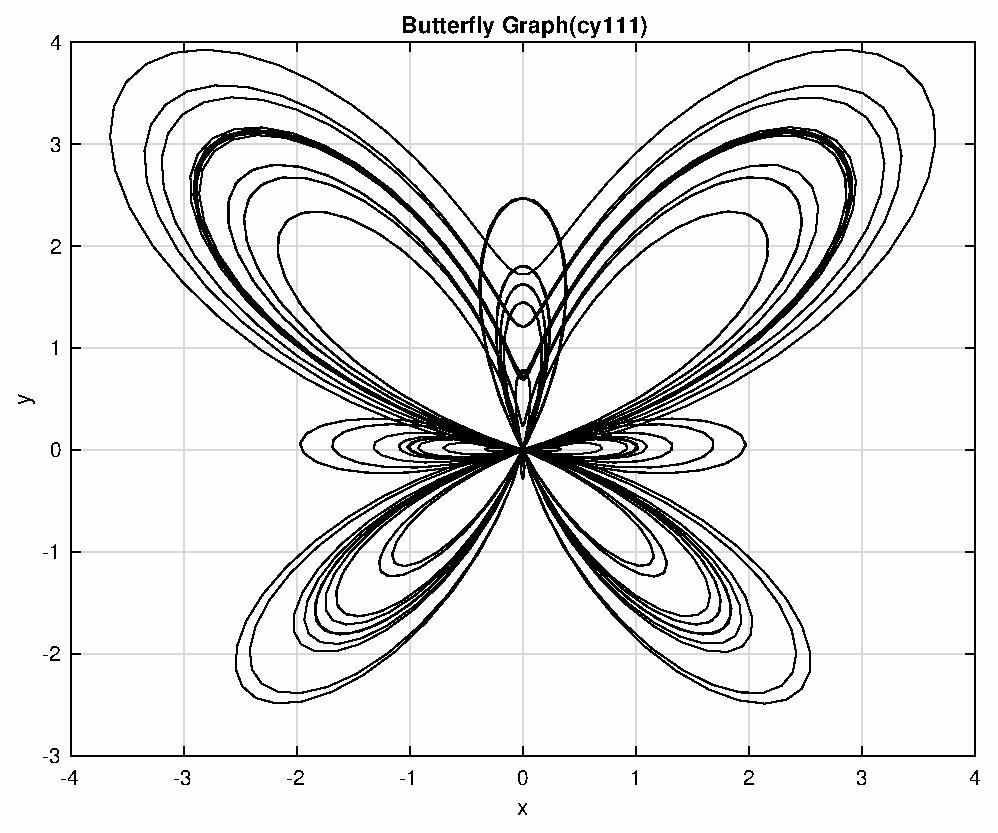
\epsfig{file=ButterflyPlot.eps, width=4.5in}
\caption{Butterfly Curve.\label{ButterflyGraph}}
\end{center}
\end{figure}

\begin{figure}[ht!]
\begin{center}
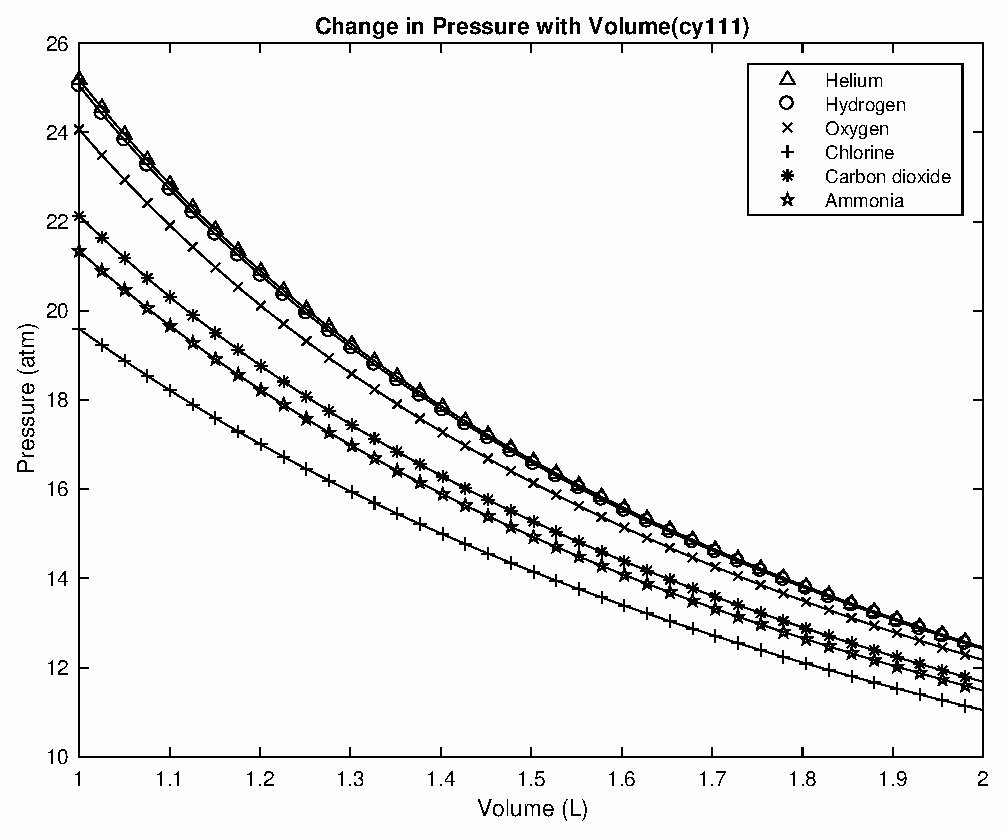
\epsfig{file=PressuresPlot.eps, width=4.5in}
\caption{VanDerWaals Calculations Plots.\label{PressureGraph}}
\end{center}
\end{figure}

\begin{figure}[ht!]
\begin{center}
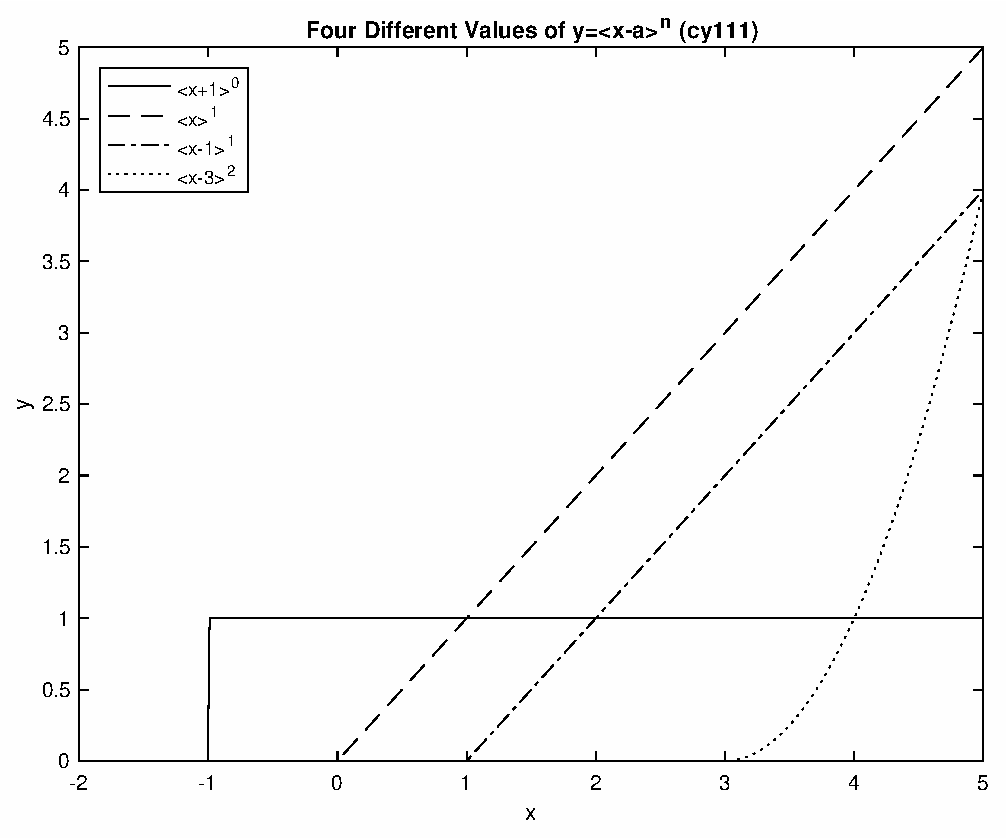
\epsfig{file=SingPlots.eps, width=4.5in}
\caption{Test of Singularity function.}
\end{center}
\end{figure}

\begin{figure}[ht!]
\begin{center}
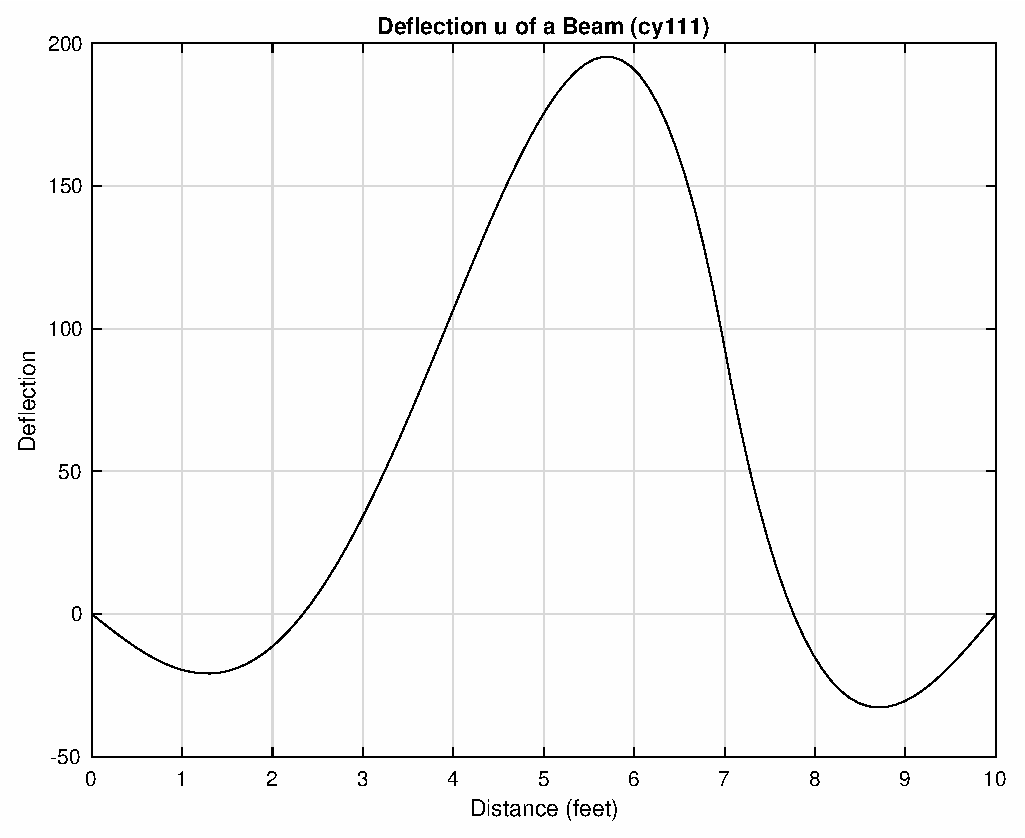
\epsfig{file=DisplacementPlot.eps, width=4.5in}
\caption{Displacement plot for a beam.}
\end{center}
\end{figure}
\clearpage

\begin{thebibliography}{9}
\bibitem{Chapra}
  Chapra, Steven C.,
  {\it Applied Numerical Methods with MATLAB for Engineering and Scientists}.
  McGraw-Hill, New York,
  3rd Edition,
  2012.
\bibitem{Palm}
  Palm, William J.,
  {\it Introduction to MATLAB for Engineers}.
  McGraw-Hill, New York,
  3rd Edition,
  2011.
\bibitem{LibreTexts}
   {\it Van Der Waal's Constants for Real Gases.} 
   Chemistry LibreTexts. 
   UC Davis, California,
   10 Aug. 2016. Web. 25 Sept. 2016.
\end{thebibliography}

\end{document}
